% \section{Results}
\begin{figure}[ht]
  \centering
  \resizebox{\columnwidth}{!}{%
  \begin{minipage}{\textwidth} %

  %----------------------------
  % First row: NO FIXATION
  \begin{subfigure}[t]{\textwidth}
    \centering
    % Left minipage for row label (empty caption)
    \begin{minipage}[b]{0.04\textwidth}
      \caption{}
      \label{fig:dynamics:no-fixation}
    \end{minipage}
    % Six images (columns)
    \begin{minipage}[b]{0.15\textwidth}
      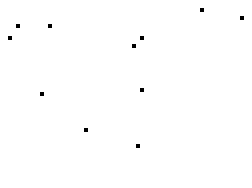
\includegraphics[width=\linewidth]{binder/binder-wse-denovo-spatial2d-explicitsite-timeseries.ipynb/binder/wse-denovo-spatial2d-explicitsite-timeseries/a=traitframes+nmut=14+rep=39a89ca6-a1b5-4b32-ae5f-f0dbb40ba027/dstream_Tbar=000504+ext=.png}
    \end{minipage}
    \begin{minipage}[b]{0.15\textwidth}
      \includegraphics[width=\linewidth]{binder/binder-wse-denovo-spatial2d-explicitsite-timeseries.ipynb/binder/wse-denovo-spatial2d-explicitsite-timeseries/a=traitframes+nmut=14+rep=5dc8e084-0382-4d7b-9b76-6c3902ca3c1d/dstream_Tbar=000952+ext=.png}
    \end{minipage}
    \begin{minipage}[b]{0.15\textwidth}
      \includegraphics[width=\linewidth]{binder/binder-wse-denovo-spatial2d-explicitsite-timeseries.ipynb/binder/wse-denovo-spatial2d-explicitsite-timeseries/a=traitframes+nmut=14+rep=5dc8e084-0382-4d7b-9b76-6c3902ca3c1d/dstream_Tbar=001400+ext=.png}
    \end{minipage}
    \begin{minipage}[b]{0.15\textwidth}
      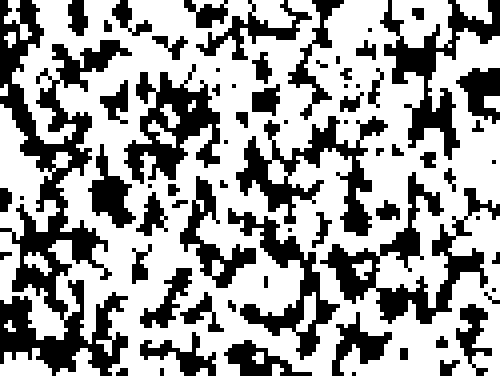
\includegraphics[width=\linewidth]{binder/binder-wse-denovo-spatial2d-explicitsite-timeseries.ipynb/binder/wse-denovo-spatial2d-explicitsite-timeseries/a=traitframes+nmut=14+rep=5dc8e084-0382-4d7b-9b76-6c3902ca3c1d/dstream_Tbar=002552+ext=.png}
    \end{minipage}
    \begin{minipage}[b]{0.15\textwidth}
      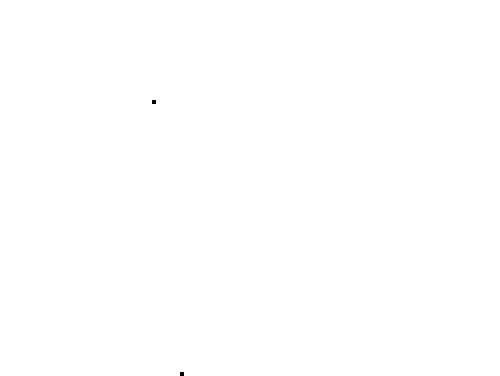
\includegraphics[width=\linewidth]{binder/binder-wse-denovo-spatial2d-explicitsite-timeseries.ipynb/binder/wse-denovo-spatial2d-explicitsite-timeseries/a=traitframes+nmut=14+rep=5dc8e084-0382-4d7b-9b76-6c3902ca3c1d/dstream_Tbar=020472+ext=.png}
    \end{minipage}
    \begin{minipage}[b]{0.15\textwidth}
      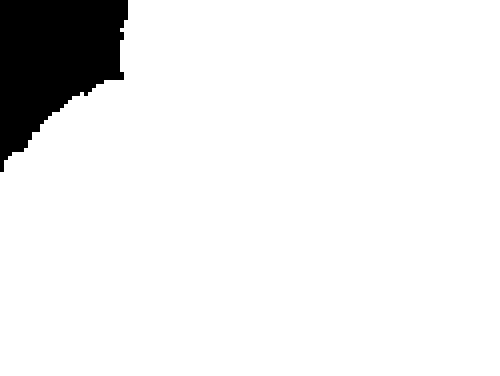
\includegraphics[width=\linewidth]{binder/binder-wse-denovo-spatial2d-explicitsite-timeseries.ipynb/binder/wse-denovo-spatial2d-explicitsite-timeseries/a=traitframes+nmut=14+rep=5dc8e084-0382-4d7b-9b76-6c3902ca3c1d/dstream_Tbar=061424+ext=.png}
    \end{minipage}
  \end{subfigure}

  \vspace{1em} % vertical space between rows

  %----------------------------
  % Second row: FIXATION
  \begin{subfigure}[t]{\textwidth}
    \centering
    % Left minipage for row label (empty caption)
    \begin{minipage}[b]{0.05\textwidth}
      \caption{}
      \label{fig:dynamics:fixation}
    \end{minipage}
    % Six images (columns)
    \begin{minipage}[b]{0.15\textwidth}
      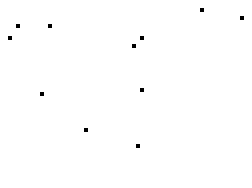
\includegraphics[width=\linewidth]{binder/binder-wse-denovo-spatial2d-explicitsite-timeseries.ipynb/binder/wse-denovo-spatial2d-explicitsite-timeseries/a=traitframes+nmut=14+rep=39a89ca6-a1b5-4b32-ae5f-f0dbb40ba027/dstream_Tbar=000504+ext=.png}
    \end{minipage}
    \begin{minipage}[b]{0.15\textwidth}
      \includegraphics[width=\linewidth]{binder/binder-wse-denovo-spatial2d-explicitsite-timeseries.ipynb/binder/wse-denovo-spatial2d-explicitsite-timeseries/a=traitframes+nmut=14+rep=39a89ca6-a1b5-4b32-ae5f-f0dbb40ba027/dstream_Tbar=000952+ext=.png}
    \end{minipage}
    \begin{minipage}[b]{0.15\textwidth}
      \includegraphics[width=\linewidth]{binder/binder-wse-denovo-spatial2d-explicitsite-timeseries.ipynb/binder/wse-denovo-spatial2d-explicitsite-timeseries/a=traitframes+nmut=14+rep=39a89ca6-a1b5-4b32-ae5f-f0dbb40ba027/dstream_Tbar=001400+ext=.png}
    \end{minipage}
    \begin{minipage}[b]{0.15\textwidth}
      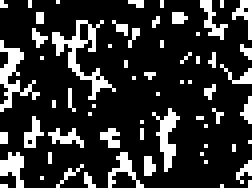
\includegraphics[width=\linewidth]{binder/binder-wse-denovo-spatial2d-explicitsite-timeseries.ipynb/binder/wse-denovo-spatial2d-explicitsite-timeseries/a=traitframes+nmut=14+rep=39a89ca6-a1b5-4b32-ae5f-f0dbb40ba027/dstream_Tbar=002489+ext=.png}
    \end{minipage}
    \begin{minipage}[b]{0.15\textwidth}
      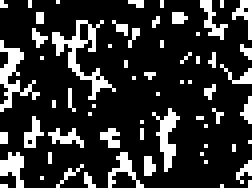
\includegraphics[width=\linewidth]{binder/binder-wse-denovo-spatial2d-explicitsite-timeseries.ipynb/binder/wse-denovo-spatial2d-explicitsite-timeseries/a=traitframes+nmut=14+rep=39a89ca6-a1b5-4b32-ae5f-f0dbb40ba027/dstream_Tbar=002489+ext=.png}
    \end{minipage}
    \begin{minipage}[b]{0.15\textwidth}
      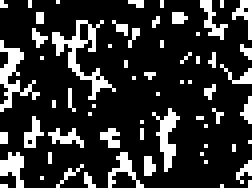
\includegraphics[width=\linewidth]{binder/binder-wse-denovo-spatial2d-explicitsite-timeseries.ipynb/binder/wse-denovo-spatial2d-explicitsite-timeseries/a=traitframes+nmut=14+rep=39a89ca6-a1b5-4b32-ae5f-f0dbb40ba027/dstream_Tbar=002489+ext=.png}
    \end{minipage}
  \end{subfigure}

  %----------------------------
  % Timepoint labels below the bottom row:
  \begin{minipage}[c]{0.154\textwidth}
\hfill
\begin{varwidth}{\textwidth}
$T = 504$
\end{varwidth}
\hfill
  \end{minipage}
  \begin{minipage}[c]{0.154\textwidth}
\hfill
\begin{varwidth}{\textwidth}
$T = 952$
\end{varwidth}
\hfill
  \end{minipage}
  \begin{minipage}[c]{0.154\textwidth}
\hfill
\begin{varwidth}{\textwidth}
$T = 1,400$
\end{varwidth}
\hfill
  \end{minipage}
  \begin{minipage}[c]{0.154\textwidth}
\hfill
\begin{varwidth}{\textwidth}
$T = 2,552$
\end{varwidth}
\hfill
  \end{minipage}
  \begin{minipage}[c]{0.154\textwidth}
\hfill
\begin{varwidth}{\textwidth}
$T = 20,472$
\end{varwidth}
\hfill
  \end{minipage}
  \begin{minipage}[c]{0.154\textwidth}
\hfill
\begin{varwidth}{\textwidth}
$T = 61,424$
\end{varwidth}
\hfill
  \end{minipage}

  \end{minipage}%
  }%

  \caption{
  \textbf{Spatiotemporal composition of simulated populations from Wafer-Scale Engine experiments.}
  \footnotesize
  Snapshots show 191 million agent populations with 2D spatial structure, using site-explicit genome model configured to adaptive potential of 14 beneficial mutations available and mutators introduced \textit{de novo}.
  Raster values are binary, with white pixels indicating a sampled nonmutators and black pixels indicating a sampled mutator.
  Subpanels \ref{fig:dynamics:no-fixation} and       \ref{fig:dynamics:fixation} show replicates where mutators do not, and do, reach fixation, respectively.
  Animations are provided at \url{https://hopth.ru/ej} and \url{https://hopth.ru/ek}.
  Example timecourses for simulations with 12 and 16 beneficial mutations available can be found at \url{https://hopth.ru/el} and \url{https://hopth.ru/em}.
  }
  \label{fig:dynamics}
\end{figure}


\section{On-device Data Management}
\label{sec:dynamics}

% Transient dynamics
% % While this scheme allowed maximization of on-device resources, as a consequence the set of sampled time points varied depending on how long nonmutator alleles persisted.
% % As a result, the number of generations elapsed per frame in provided animations varies.

% To assess how competition between non- and mutator strains unfolds at very large population scales, we performed an additional set of simulations on the WSE using the site-explicit model of adaptation, where mutators originated \textit{de novo} from nonmutator strains.
% For these experiments, a subpopulation size of 256 agents per PE was used to preserve on-device memory to record time series data.
% This configuration yielded a net population size of 191 million agents.
% In these trials, we probed the critical region where outcomes transition between nonmutator and mutator fixation, configuring adaptive potential between 12 and 16 available beneficial mutations.

A key challenge in this work was balancing limited on-device memory between simulation content and data recording.
For example, some experiments required time series measurements of mutator prevalence in PE subpopulations (Figure \ref{fig:dynamics}).
To economize memory use, we applied recently-developed algorithms that generalize ring buffer storage to efficiently perform systematic temporal downsampling \citep{moreno2024algorithms,gunther2014algorithm}.
Successive local samples are recorded as single bits within a flat, fixed-size buffer --- with no bookkeeping overhead.
Crucially, because recording duration (i.e., until extinction) is unknown \textit{a priori}, this approach dynamically coarsens recording density via overwrites once storage capacity is reached --- strictly bounding memory use.

% Crucially, given extinction timings are unknown \textit{a priori}, after storage capacity is reached, this approach  a representative online downsample, of configurable composition, is dynamically coarsened once capacity is reached.
% We configured each processor element to sample a genome from its local population and record its mutator allele status (i.e., a binary value as either a non- or mutator).
% However, the duration of recording was not known \textit{a priori}, as it depended on the timing of stochastic fixation events within the simulation itself.
% To efficiently curate this single-bit data within per-PE memory limits while allowing  (as timing of extinction or fixation events is not known \textit{a priori}), we leveraged recently introduced ``DStream'' ring buffer data structures \citep{moreno2024algorithms}.
% Crucially, this approach constrained memory use to a fixed-size buffer known \text{a priori}, while allowing recording to be dynamically halted when nonmutators were determined to be locally extinct (and restarted if they are reintroduced).
% These allowed to be stored in flat memory without data structure overhead, with configurable distribution over time.
Among other results, this data collection strategy revealed that even in circumstances where mutator alleles did not reliably fix, they could nonetheless transiently dominate population composition --- in some cases, reaching peaks upwards of 99.9\% frequency.
% at peak mutator prevalence, nonmutators transiently shrink to less than 0.1\% of population in experiments under conditions where mutators were initially rare but did not fix.
% Given that biological analyses often amenable to incomplete data,

Given limitations in studying real-world systems, biological analyses are often robust to coarsening and sampling.
As such, we see significant opportunity in future work to more broadly explore how such best-effort data collection approaches can be applied to meet practical constraints of hardware accelerator device architectures.
%  which we are interested in continuing to explore in future work.
%Owing to rich statistical methods developed to overcome incomplete data in studying real-world systems,

% Figure \ref{fig:dynamics} arranges sequential population snapshots from two example simulations, both with adaptive potential of 14 beneficial mutations.
% In the first example, mutators fixed; in the second, they did not.
% At outset, panels \ref{fig:dynamics:no-fixation} and \ref{fig:dynamics:fixation} unfold similarly.
% First, mutator strains appear \textit{de novo} across the breadth of simulated populations.
% Then, as patches of mutators expand outwards, the nonmutator population is broken into pockets.
% % Mutator strains continued to stem from nonmutator lineages as they accrued adaptive mutations.
% % Of 16 replicates where we observed mutators fix, we found 2 cases where the final dominant mutator lineage arose from a partially adapted nonmutator lineage --- harboring 1 and 3 beneficial mutations, respectively.
% % https://github.com/mmore500/hypermutator-dynamics/blob/90422b30f2dd9ca29baad273cbcc676dbfeab55f/binder/wse-denovo-spatial2d-explicitsite-genomes.ipynb
% In scenarios where mutators fix, surviving patches of nonmutators dwindle away entirely (panel \ref{fig:dynamics:fixation}).
% Where nonmutators persist, they re-establish via concentric growth from surviving pockets (panel \ref{fig:dynamics:no-fixation}).
% This TODO allowed us to assess the fact that mutators transiently peak at well above the majority of population composition.
% \input{fig/peaksweep}


\section{On-device Performance}
\label{sec:performance}

\begin{figure}

% \begin{subfigure}{0.5\textwidth}
% 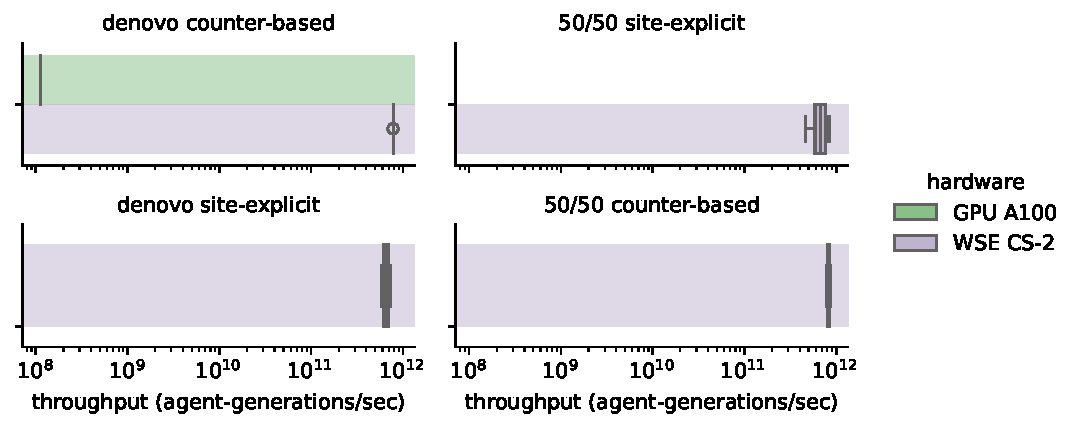
\includegraphics[width=\textwidth, trim={0cm 0cm 2.5cm 0cm}, clip]{binder/binder-perf-wse-vs-gpu.ipynb/binder/teeplots/col=experiment-design+hue=hardware+orient=h+viz=backplot+x=throughput-agent-generations-sec+ext=.pdf}
% \caption{throughput}
% \label{fig:perf:throughput}
% \end{subfigure}%
% \begin{subfigure}{0.49\textwidth}
\centering
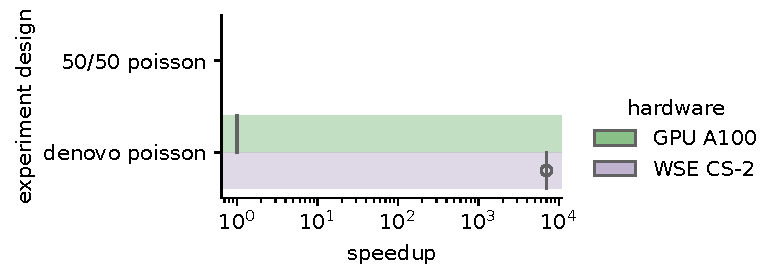
\includegraphics[width=0.85\linewidth]{binder/binder-perf-wse-vs-gpu.ipynb/binder/teeplots/hue=hardware+orient=h+viz=backplot+x=speedup+y=experiment-design+ext=.pdf}

\vspace{-2ex}
% ~
% \caption{speedup}
% \label{fig:perf:speedup}
% \end{subfigure}

\caption{
  \textbf{CPU, GPU, and WSE simulation performance.}
  \footnotesize
  CPU throughput was measured from NumPy-backed simulation code, GPU throughput was measured from equivalent CuPy-backed simulation code, and WSE throughput was measured from a comparable Cerebras Software Language implementation.
  CPU experiments were single-core on AMD EPYC 7H12 (2.595 GHz), GPU hardware was NVIDIA A100 hosted by AMD EPYC 7713 (2.0 GHz) or Intel Xeon 8358 (2.6 GHz), and WSE hardware was CS-2 hosted by Intel Xeon Platinum 8280L (2.7-4.0 GHz).
  Speedup was calculated relative to mean CPU throughput.
  % Shaded areas indicate bootstrapped 95\% confidence intervals with sample size $\geq 10$.
}
\label{fig:perf}
\end{figure}


To assess the efficacy of hardware accelerator resources in expediting our simulations, we collected timings of runtime duration from our simulation experiments.
As a baseline comparison point, we also benchmarked corresponding single-core CPU simulation code.

Mean throughput was 7.0 (SD 0.5) million agent-generations per second (AGPS) on CPU, 2.7 (SD 0.03) billion AGPS on GPU, and 780 (SD 0.5) billion AGPS on WSE for \textit{de novo} trials using the counter-based model.
We found that WSE provided a speedup of $111,091\times$ (SD 75) over CPU and $294\times$ (SD 0.2) over GPU (Figure \ref{fig:perf}).
% Net speedup, normalized to mean CPU throughput, was $378\times$ (SD 4) on GPU and $111,091\times$ (SD 75) on WSE.
% Normalized to GPU performance, WSE provided a speedup of $294\times$ (SD 0.2).

% Under the site-explicit model, WSE gave 650 (SD 50) billion AGPS under \textit{de novo} conditions.
% The site-explicit model was not implemented on GPU.
% For all the above, 50/50 trials gave similar performance to \textit{de novo}.

On WSE, we found agent-generation throughput to be consistent across per-PE population densities.
%, as shown in Supplementary Figure \ref{fig:perf-tilepop}.
In contrast, on GPU we encountered an apparent memory-wall effect where mean  throughput dropped $>95\%$ to 121 million AGPS when increasing net population size from 15.1 million to 175 million.
% For this reason, we only scaled GPU experiments up to 15.1-million-agent populations ($243 \times 243$ demes).

% \subsection{Major Results}

% In our initial experiment, we confirmed that large populations favor mutator fixation, under the assumption of unlimited adaptive potential.
% Consistent with expectations, we found that restricting adaptive potential by capping available adaptive mutations reversed outcomes in large populations to favor nonmutators.
% Investigating the influence of population structure and composition, we found spatial structure to substantially increase the amount of adaptive potential required to fix mutator alleles in large populations.
% However, this effect only occurred when mutator alleles were initially rare within the population.
% We also report qualitative differences between effects of population size on mutator fixation probability under well-mixed versus 2D population structure when mutations are rare.
% In the final part of our investigation, we analyze the spatiotemporal dynamics of our simulations to better understand the mechanisms at play behind these effects.

% Differing from existing results, we find that in the situation of limited adaptive potential, the effect of population structure on fixation probability is actually opposite to that predicted under the theory.
% Population structure has also been found to influence mutator outcomes, with deviation from well-mixed conditions being linked to a higher probability for hypermutator fixation so long as any connectivity remains between subpopulations \citep{raynes2019migration}.


% \section{Results and Discussion} \label{sec:results}

% In this work, we investigate the interactions between population size, adaptive potential, and population structure in influencing selection on mutator traits within asexual populations.
% In our first experiments, we replicate previous work by \citet{raynes2018sign} showing sign-change effects of population size on mutator favorability.
% Subsequent experiments investigate how these dynamics vary based on initial mutator abundance and the availability of beneficial mutations.
% Finally, experiments compare mutator dynamics between well-mixed population structure and spatial segregation into subpopulations connected by migration.

% \subsection{Scaling Population Size}
% \label{sec:scaling-population-size}

% In a first set of experiments, we tested the capability of our model to reproduce the qualitative regimes of mutator dynamics across population scales identified by \citet{raynes2018sign}.
% In the first regime, where population size is very small, fixation of mutator and nonmutator alleles is nearly equiprobable, owing to the overwhelming influence of stochastic effects.
% Subsequently, in medium-sized populations, mutators become disfavored on account of increased power of selection becoming in penalizing the increased mutational load imposed by mutator allelees.
% Finally, in sufficiently large populations, a sign-change fitness effect occurs and mutator fixation becomes overwhelmingly favored.
% This effect occurs in asexual populations because population size increases the probability of at least one mutator discovering a beneficial mutation, and so ``hitch-hiking'' to sweep out nonmutators.

% \begin{figure}[h]
  % adapted from https://tex.stackexchange.com/a/122813/316176
  \captionsetup[subfigure]{justification=raggedright}
  \begin{minipage}{0.7\textwidth}

    \begin{minipage}{0.04\textwidth}~\end{minipage}%
    \begin{minipage}{0.44\textwidth}
      \centering
      \itshape
      \textbf{unlimited} beneficial mutations
    \end{minipage}%
    \begin{minipage}{0.34\textwidth}
      \centering
      \itshape
      \textbf{single} beneficial mutation
    \end{minipage}

    ~\vspace{-1.5ex}

    % Top subfigure
    \begin{subfigure}[b]{\linewidth}
      \begin{minipage}{0.88\textwidth}
        \begin{minipage}{0.53\textwidth}
          \includegraphics[height=2.9cm, trim={0cm 0.2cm 3.5cm 0.8cm}, clip]{binder/binder-wse-5050-spatial2d-32atile-infben-traits.ipynb/binder/teeplots/wse-5050-spatial2d-32atile-infben-traits/errorbar=ci+hue=genotype+num-abm=(inf,)+style=genotype+viz=size-fixation-areaplot+x=population-size+y=fixation-probability+ext=.pdf}%
        \end{minipage}%
        \begin{minipage}{0.47\textwidth}
          \includegraphics[height=2.9cm, trim={1.3cm 0.2cm 3.5cm 0.8cm}, clip]{binder/binder-wse-5050-spatial2d-32atile-infben-traits.ipynb/binder/teeplots/wse-5050-spatial2d-32atile-infben-traits/errorbar=ci+hue=genotype+num-abm=(1.0,)+style=genotype+viz=size-fixation-areaplot+x=population-size+y=fixation-probability+ext=.pdf}
        \end{minipage}
      \end{minipage}%
      \hspace{-3ex}%
      \begin{minipage}{0.12\textwidth}
        \raggedright
        \caption{\footnotesize 32 agents per PE\\~\\~\\}
        \label{fig:wse-inf-one:32}
      \end{minipage}%
    \end{subfigure}%

    % Bottom subfigure - Adjusted layout to match the top
    \begin{subfigure}[b]{\linewidth}
      \begin{minipage}{0.88\textwidth}
        \begin{minipage}{0.53\textwidth}
          \includegraphics[height=2.9cm, trim={0cm 0.2cm 3.7cm 0.8cm}, clip]{binder/binder-wse-5050-spatial2d-2048atile-infben-traits.ipynb/binder/teeplots/wse-5050-spatial2d-2048atile-infben-traits/errorbar=ci+hue=genotype+num-abm=(inf,)+style=genotype+viz=size-fixation-areaplot+x=population-size+y=fixation-probability+ext=.pdf}%
        \end{minipage}%
        \begin{minipage}{0.47\textwidth}
          \includegraphics[height=2.9cm, trim={1.3cm 0.2cm 3.7cm 0.8cm}, clip]{binder/binder-wse-5050-spatial2d-2048atile-infben-traits.ipynb/binder/teeplots/wse-5050-spatial2d-2048atile-infben-traits/errorbar=ci+hue=genotype+num-abm=(1.0,)+style=genotype+viz=size-fixation-areaplot+x=population-size+y=fixation-probability+ext=.pdf}
        \end{minipage}
      \end{minipage}%
      \hspace{-3ex}%
      \begin{minipage}{0.1\textwidth}
        \caption{\footnotesize 2,048 agents per PE\\~\\~\\}
        \label{fig:wse-inf-one:2048}
      \end{minipage}%
    \end{subfigure}%

~\vspace{-1.2ex}

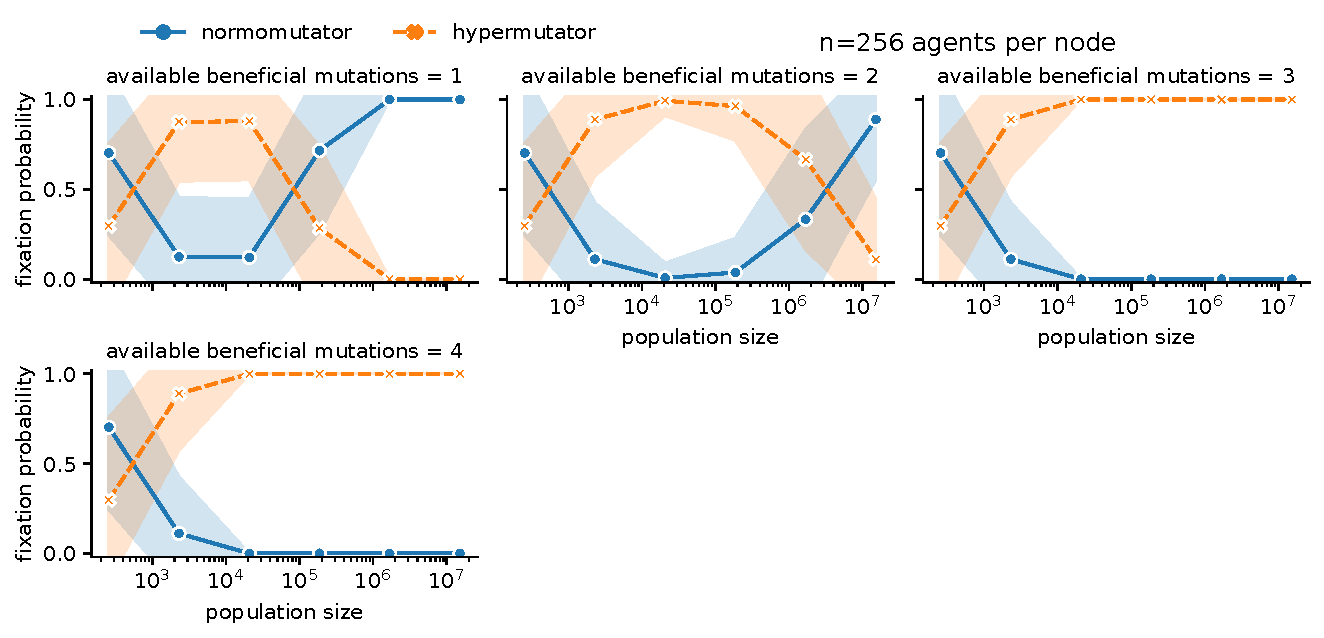
\includegraphics[width=0.9\textwidth, trim={0cm 4.7cm 6.2cm 0cm}, clip]{binder/binder-wse-5050-spatial2d-2048atile-infben-traits.ipynb/binder/teeplots/wse-5050-spatial2d-2048atile-infben-traits/col=available-beneficial-mutations+errorbar=sd+hue=genotype+kind=line+style=genotype+viz=relplot+x=population-size+y=fixation-probability+ext=}

  \end{minipage}%
  \begin{minipage}{0.3\textwidth}
    \caption{%
      \textbf{Restricted adaptive potential favors nonmutators in large populations.}
      \footnotesize
      Area plots compare mutator versus nonmutator fixation probabilities across surveyed population sizes.
      When adaptive potential is unlimited (left column), mutators are strongly favored in large populations, owing to their capacity to more rapidly discover beneficial mutations.
      Right column shows fixation outcomes across population sizes, with adaptive potential restricted to just one beneficial mutation.
      As before, mutators gain favor in intermediate population sizes.
      However, under the adaptation-restricted regime, nonmutators regain favor at very large population sizes.
      Top panel, \ref{fig:wse-inf-one:32}, shows results with subpopulation size of 32 agents per PE, scaling population size up to 23.9 million.
      Bottom panel, \ref{fig:wse-inf-one:2048}, reports 2,048 agents per PE with population sizes up to 1.5 billion.
      Experiments were conducted on WSE with counter-based genome model, using populations initialized with a 50/50 mix of non- and mutators.
      Error bands indicate bootstrapped 95\% confidence intervals.
      Supplementary Figure \ref{fig:fixheat-wse-altatile} details results in a tabular format.
    }
    \label{fig:wse-inf-one}
  \end{minipage}
\end{figure}


% As shown in the left panel of Figure \ref{fig:wse-inf-one:32}, our simulations reproduce the sign-change fitness effect described by \citet{raynes2018sign}.
% Leveraging the capabilities of WSE accelerator hardware, we tested population sizes several orders of magnitude beyond those reported in \citet{raynes2018sign}.
% For these experiments, 2D population structure was used with 50/50 initialization.
% In line with expectations, no further qualitative differences in mutator fixation probability emerged in these larger population sizes, which ranged up to 1 billion agents.
% For the largest-scale trials, shown in the left panel of Figure \ref{fig:wse-inf-one:2048}, an increased subpopulation size of 2,048 agents per deme was used.
% As such, in these trials, note that coarsened spacing between surveyed population sizes obscures the sign-change fitness effect near the lower bound of population size.

% \subsection{Restricting Adaptive Potential}
% \label{sec:restricting-adaptive-potential}

% \subsection{Major Results}

% \begin{figure*}

\begin{minipage}{0.65\textwidth}
  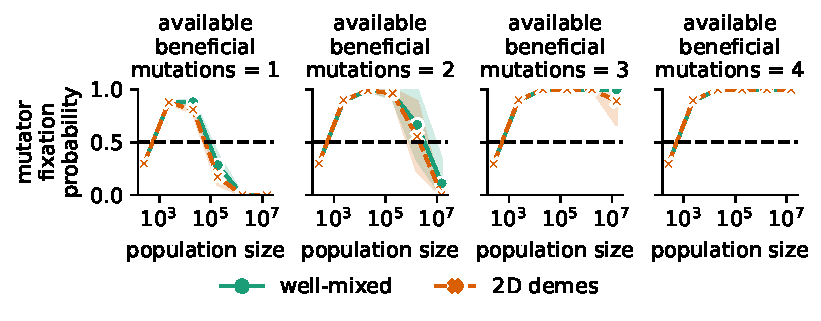
\includegraphics[width=\textwidth]{binder/binder-cupy-5050-traits.ipynb/binder/teeplots/cupy-5050-traits/col=available-beneficial-mutations+errorbar=ci+hue=population-structure+kind=line+palette=dark2+style=population-structure+viz=relplot+x=population-size+y=fixation-probability+ext=.pdf}%
\end{minipage}
\begin{minipage}{0.3\textwidth}
\caption{
\textbf{Well-mixed and spatially-structured populations exhibit similar relationship between population size and mutator fixation probability.}
\footnotesize
In both scenarios, as available beneficial mutations are increased, mutators gain favor in progressively larger population sizes.
Simulations were conducted on GPU using the counter-based genome model, with populations initialized to a 50/50 mix of non- and mutators.
Subpopulations comprised 256 agents per PE.
Shaded bands show bootstrapped 95\% confidence intervals.
}
\label{fig:avail-ben-muts-gen}
\end{minipage}

\end{figure*}


% Given that experiments conducted on the WSE platform all involve 2D spatial structure, we implemented an additional set of GPU-based experiments to compare findings with well-mixed population structure.
% Figure \ref{fig:avail-ben-muts-gen} overviews these results.
% Although experiments ranged up to a smaller maximum population size on the GPU platform, detected regimes of mutator dynamics are consistent with WSE-based experiments.
% Comparing on the basis of spatial structure, we find fixation probabilities to be near-identical between GPU-based trials using 2D and well-mixed structure across surveyed conditions.
% % https://github.com/mmore500/hypermutator-dynamics/blob/484ac79f35baf10e4acc52babee836d10ab50bdb/binder/cupy-5050-traits.ipynb
% We find significant divergence in fixation probability between spatial structure treatments only for population size 20,736 with adaptive potential of one available beneficial mutation (Mann-Whitney U test; $p < 0.0005$; Bonferroni corrected $p < 0.01$).

% \subsection{Effects of Background Mutator Prevalence}
% \label{sec:background-hypermutator-prevalence}

% \input{fig/denovo-5050-conditions-combined}

% Having observed large population size prevent mutator fixation in competition experiments under conditions of limited adaptive potential, we next sought to assess how such an effect might manifest in more naturalistic conditions.
% For this purpose, we relaxed the initial condition that mutators begin ``50/50'' in equal proportion to nonmutators.
% Instead, we allowed mutators to enter the population at a low background rate \citep{desai2011balance,johnson1999approach}, an experimental design common with several previous simulation studies of hypermutator dynamics \citep{wylie2009fixation,tenaillon1999mutators}.
% To provide a conservative reflection of the impact of mutator allele rarity, we used a mutator allele introduction probability of $10^{-6}$ per replication event.
% Figure \ref{fig:denovo-5050-conditions-combined} compares mutator fixation probabilities between 50/50 and \textit{de novo} conditions.
% Trials were conducted with 2D spatial structure on the WSE platform.
% With 256 agents per deme, population size scaled up to 136 million agents.

% Prior work analyzing conditions with infinite adaptive potential has shown per-capita favorability of mutator traits to be density independent \citep{raynes2019selection}.
% As such, a lower background rate for mutator alleles should be expected to substantially reduce the net probability of mutator fixation.
% In line with expectations, the \textit{de novo} treatment substantially reduces mutator fixation.
% Under \textit{de novo} conditions, nonmutators reliably resist mutator fixation in populations of 136 million through more than 10 beneficial mutations available.
% Under 50/50 conditions, by contrast, mutators begin to fix in these large populations past 2 beneficial mutations available.

% We performed sensitivity analysis of our findings to the underlying counter-based genome model used.
% For this purpose, we implemented an alternate ``site-explicit'' model where the probability of discovering a beneficial mutation scales proportional to the number available.
% As shown in Supplementary Figure \ref{fig:wse-site-explicit-counter-based}, results were generally consistent between the two genome models.
% Notably, though, under the ``site-explicit'' model, mutator alleles are more frequently fixed within the smallest surveyed population size under 50/50 initialization.

% % ^^^ https://github.com/mmore500/hypermutator-dynamics/blob/5e904ac2fbbd4b41a0ad679883fc1a63af71c00c/binder/wse-denovo-spatial2d-explicitsite-timeseries.ipynb
% To assess the magnitude of transient peak mutator concentrations across levels of adaptive potential, we performed an additional set of four-replicate simulations with adaptive potentials ranging from 2 to 10 available beneficial mutations.
% For all replicates with 6 or more available beneficial mutations, mutators peaked beyond 50\% prevalence (Figure \ref{fig:peaksweep}).

% \subsection{Effects of Population Structure}
% \label{sec:population-structure}

% In a final set of experiments, we extended our earlier trials with 50/50 initialization to assess the impact of spatial structure on mutator dynamics where mutators are initially rare.
% In particular, we were curious whether removal of population structure would negligibly affect mutator fixation probabilities, as was earlier the case with 50/50 initialization.
% Trials conducted in this experiment comparing the 2D deme structure to fully well-mixed conditions were conducted using GPU evaluation.
% As a result, population sizes ranged only up to 15 million.

% \input{fig/spatial-structure-combined}

% Figure \ref{fig:spatial-structure-combined} plots increase in mutator fixation probability with available adaptive potential across a spectrum of population sizes.
% Interestingly, spatial structure does cause results to differ substantially under \textit{de novo} conditions.
% We find that in large nonmutator populations of 15 million with well-mixed structure, fixation probability of mutator alleles becomes appreciable with adaptive potential of only 5 available beneficial mutations.
% Thisis not the case for large populations with 2D deme structure, where fixation of mutator alleles become appreciable above 10 available beneficial mutations.
% For intermediate population sizes of 186,000 agents, however, an opposite effect occurs: spatial structure raises the probability of mutator fixation across the board of available adaptive potential compared to well-mixed conditions.

% These findings contrast with previous modeling work assuming unlimited adaptive potential, which predicts that so long as any level of connectivity exists between subpopulations, spatial structure boosts mutator fixation probability \citep{raynes2019migration}.
% One possible explanation for why spatial structure can decrease mutator fixation probability is in extending fixation times, which extends the opportunity for nonmutators to exploit available adaptive potential before being driven to extinction.
% This described effect notably aligns with findings from \textit{in vivo} evolution experiments with \textit{E. coli} that show that migration barriers delaying introduction of mutator strains into nonmutator populations can reduce mutator advantage \citep{lechat2006escherichia}.

% On a separate front, it is surprising that substantial differences in mutator dynamics between deme-structured and well-mixed conditions only become apparent with low initial mutator frequency, given the established expectation of fitness effects of mutator alleles as a density- and number- independent \citep{raynes2019selection}.
% While one possible explanation may be in part that detectability of fitness effect magnitudes is masked by sensitivity limitations of the 50/50 assay, this result draws into question the extent to which density-independence of mutator fitness effects generalizes to scenarios with limited adaptive potential and spatial structure.
% In future work, it would be informative to test whether the impact of spatial structure where mutators are rare stems from heterogeneity in the spatial distribution of mutator clades or from slowing the spread of beneficial alleles.
